\section{Product Testing}

From day one all code had to be tested frequently and thoroughly, eliminating errors and all bad test cases. Most testing had to be done with the Leshan server. A dummy client was created to simulated the end device and then HTTP request where sent from browser and tested with the android app as well.

\subsection{MQTT testing}

Testing was done on MQTT for making sure that clients could connect to it and communicate the FREE/OCCUPIED between the sensor and light device. That part worked for all teams connecting to the system. As can be seen in Figure \ref{fig:mqtt3}.
\begin{figure}[h]
	\begin{center}
		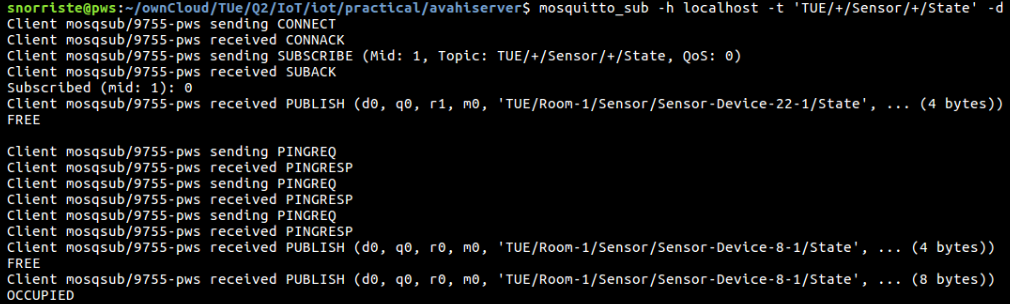
\includegraphics[width=\linewidth]{img/mqtt3}
		\caption{Mosquitto tested during Plugfest with other teams. MQTT broker works and clients can communicate.}
		\label{fig:mqtt3}
	\end{center}
\end{figure}

\subsection{Leshan Testing}

This section will show testing of Leshan, how it responded to requests and how the development interface looks like. All Figures from Leshan testing are in Appendix A due to large size. In Figure \ref{fig:observe} the log for the Leshan server is displayed when an request from the web app is made to observe a sensor value (resource 10350).

An important part to be working is the updating of ownership and thus it is useful to show the testing of the part. In Figure \ref{fig:own} the Leshan server log can be seen when the Cloud group updates the ownership via their manager web app seen in Figure \ref{fig:cloudown}.


Creating a user with password and other information accordingly can be seen in Figure \ref{fig:newuser} and \ref{fig:newusercloud}



\subsection{App Testing}
In Figure \ref{fig:app} the app can be seen working with multiple clients. The light can be controlled as indicated.

\subsection{Avahi Testing}

Avahi was tested multiple times with the red team. Figure \ref{fig:avahi} shows the command publish the service and then if the client uses the same parameters it will connect. 